\chapter{Methods}
\label{chapterlabel3}

The method of tackling this problem will be based on previous research done in this domain. There are three essential components for this project:
\begin{figure}[h]
\caption{Basic flowchart}
\centering
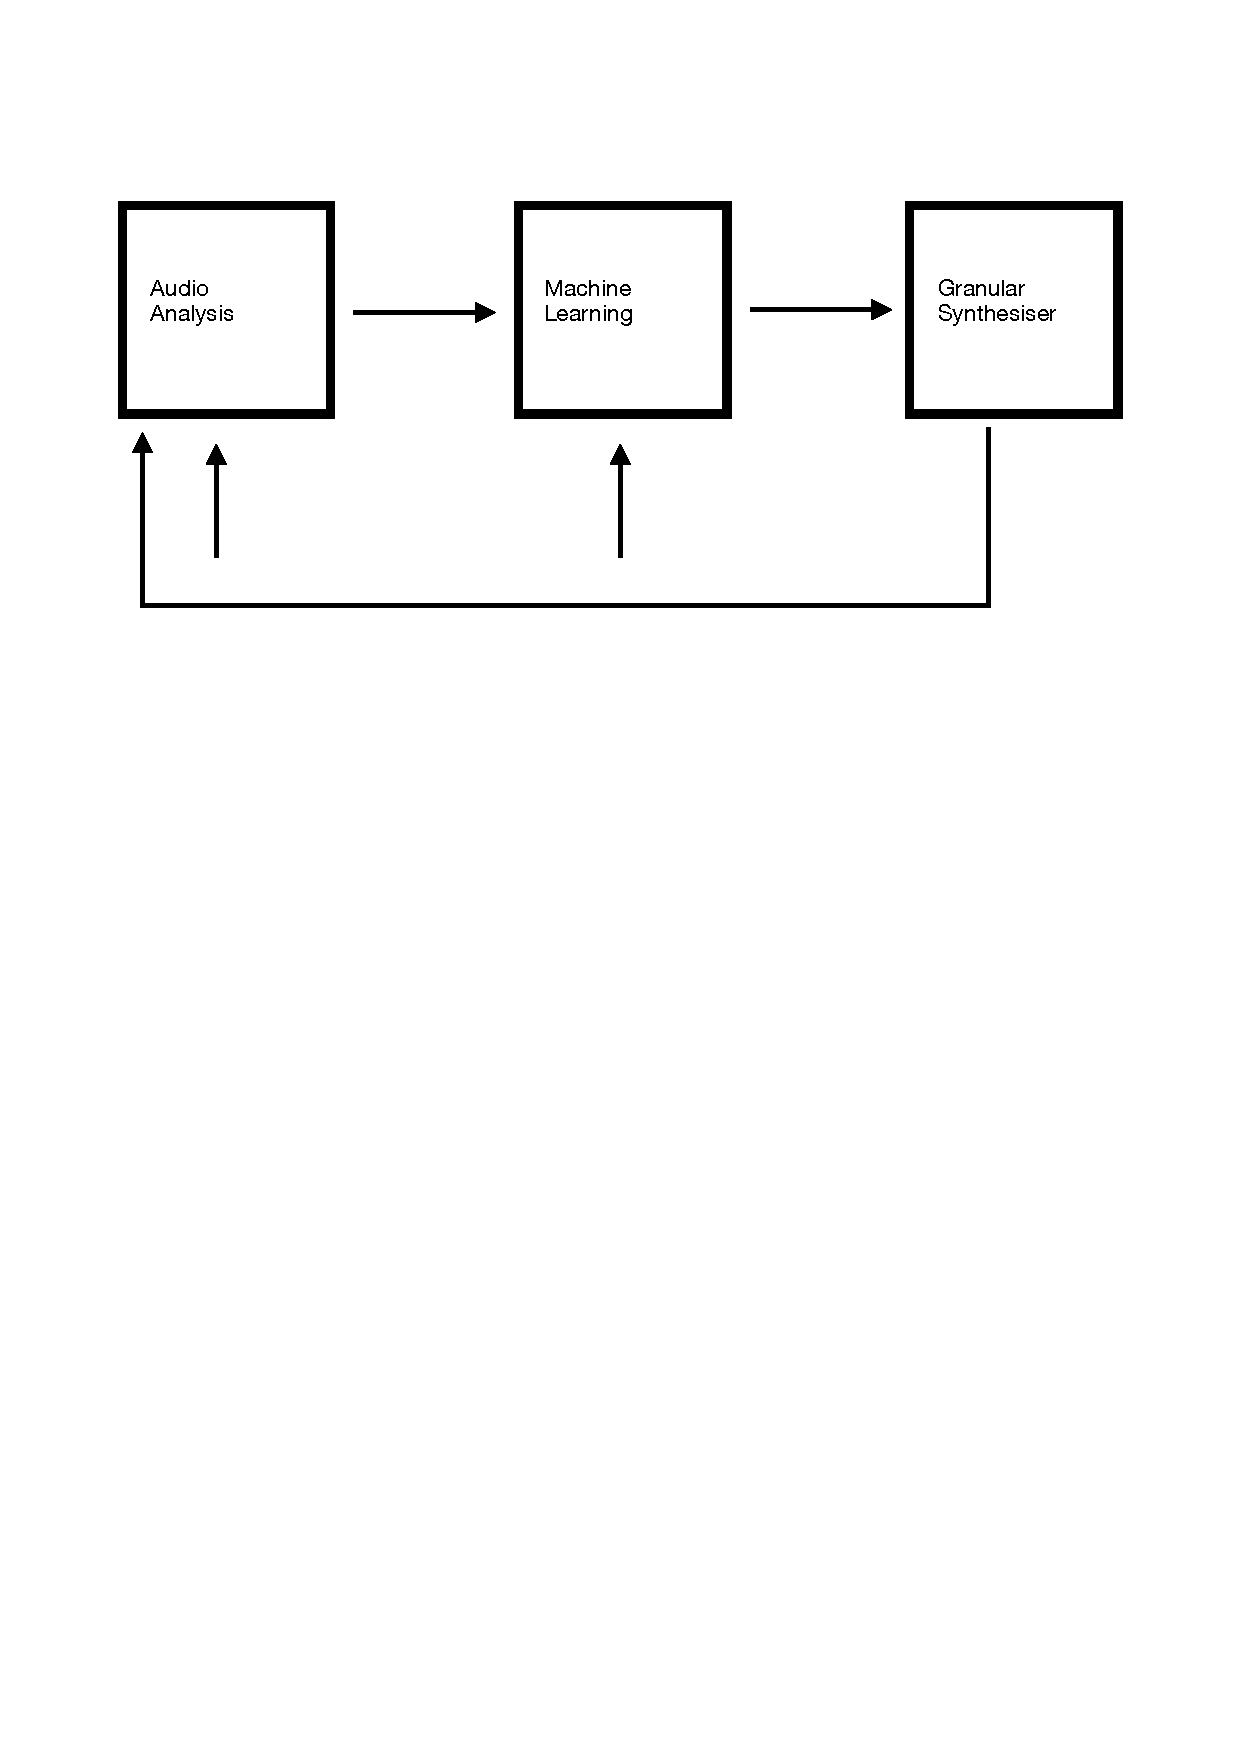
\includegraphics[width=0.5\textwidth]{images/flowchart}
\end{figure}

\section{Synthesis}

- how it is build

- what libraries etc are used

- what parameters are being manipulated

- how each parameter influences the output sound

- what sounds are being sampled (where do the grains come from)(how does the
behaviour change depending on the sample)

The box ``Granular Synthesiser'' in figure 1. represents a granular synthesizer.
It is build in C++, using the 'JUCE' framework(SOURCE). (Add about it being
quasi-synchronous, and all other possible information.)

\section{Audio descriptors}

- how it is build

- what libraries etc are used

- what testing has been done

- what descriptors influence what parameters

- how do they work (maybe briefly)

- how do they speak to the 'agent' 

The ``Audio Analysis'' box in figure 1. represents the aspect of the project
responsible for extracting audio features from input sounds. This requires some
testing in order to see which works best for this task. Feature extractors
considered are: MFCC and DBM. The environment of choice is the ``Essentia''
library for C++. (SOURCE) 

\section{Machine learning}

- how it is build

- what libraries etc are used

- how is it trained

- what data is used

``Machine Learning'' in figure 1, stands for Machine Learning. This aspect will
most likely be implemented in python, either using the
``scikit.learn''
%\cite{noauthor_scikit-learn:_nodate}
library, or the
``TensorFlow''
% \cite{noauthor_tensorflow_nodate}
library. Depending on which
Machine Learning algorithms will be used. This will be determined during
testing. The ones being considered at the moment include k-NN, Neural Networks,
and LSTM(Long Short-Term Memory Neural Network)
%\cite{yee-king_automatic_2018}.
Training of whichever algorithm chosen will be happening on data generated by
me. Vectors of synthesis engine parameter values, and audio analysis values,
possibly as a CSV file will be created. The goal here is to automate a sampled
walk through the parameter space, and extract audio features for each point.
Possibly,  a genetic algorithm could be
used for this process
% \cite{yee-king_automatic_2018}.